\appendix

\chapter{Rotating spin Hamiltonian}\label{app:rotating_spin_hamiltonian}

In Chap.~\ref{chap:2_adiabaticity} we used the example of a spin rotating in a magnetic field to illustrate adiabatic processes in quantum systems. We considered a spin starting in the $\ket{+}$ state and being rotated from the $x$ direction to the $z$ direction during some total time $\tau$ according to the Hamiltonian in Eq.~\eqref{eq:rotating_spin_H}, which I will reproduce here for convenience:
\begin{equation}\label{eq:rotating_spin_H_lambda}
    H(\lambda) = -\cos(\lambda)\sx - \sin(\lambda)\sz,
\end{equation}
with $\lambda(t) = \frac{\pi t}{2 \tau}$. The \acrref{AGP} operator ansatz $\approxAGP$ for this system can be described by the operator $\sy$ scaled by some $\lambda$-dependent coefficient which we will refer to as $\alpha(\lambda)$
\begin{equation}
    \approxAGP = \alpha(\lambda) \sy
\end{equation}
as discussed in the main text. We will now proceed to show how we can arrive at the resulting form of $\alpha$ given in Eq.~\eqref{eq:rotating_spin_alpha} using the \acrref{LCD} method outlined in Sec.~\ref{sec:2.4.1_LCD}.

The first step is to find the operator $G_{\lambda}$ given in Eq.~\eqref{eq:G_operator}:
\begin{equation}
    \begin{aligned}
        G_{\lambda}(\approxAGP) &= \dlambda H + i\comm{\approxAGP}{H} \\
        & = \sin(\lambda)\sx - \cos(\lambda)\sz + 2\alpha(\lambda)\sin(\lambda)\sx - 2\alpha(\lambda) \cos(\lambda)\sz \\
        & = (1 + 2\alpha(\lambda))\sin(\lambda) \sx - (1 + 2\alpha(\lambda))\cos(\lambda)\sz,
    \end{aligned}
\end{equation}
where we have used $\hbar = 1$. This can then be used to define the action
\begin{equation}
    \begin{aligned}
        \mathcal{S}(\approxAGP) &= \Tr\left[G^2_{\lambda}(\approxAGP) \right] \\
        & = 2 (1 + 2\alpha(\lambda))^2 \sin^2(\lambda) + 2 (1 + 2\alpha(\lambda))^2 \cos^2(\lambda) \\
        & = 2 (1 + 2\alpha(\lambda))^2.
    \end{aligned}
\end{equation}
In order to find the form of $\alpha$, we need to find the minimum of the action $\mathcal{S}(\approxAGP)$ with respect to $\alpha$, which can be easily done:
\begin{equation}
    \begin{aligned}
        \frac{\delta \mathcal{S}}{\delta \alpha} &= 8(1 + 2\alpha(\lambda)) \\
        \Rightarrow \alpha(\lambda) &= -\frac{1}{2},
    \end{aligned}
\end{equation}
which is the expected result. 

It can be checked, for this simple example, that $\approxAGP = -\frac{1}{2} \sy$ is the exact \acrref{AGP} operator $\AGP{\lambda}$ by using Eq.~\eqref{eq:AGP_adiabatic_basis} where the matrix elements of the \acrref{AGP} are written out explicitly as:
\begin{equation}
    \begin{aligned}
        \AGP{\lambda} &= i \Big(\sum_n \braket{n}{\dlambda n} \dyad{n} + \sum_{m \neq n} \ket{m} \frac{\mel{m}{\dlambda H}{n}}{(E_n - E_m)} \bra{n} \Big) \\
        & = i \Big(\sum_n \braket{n}{\dlambda n} \dyad{n} + \sum_{m \neq n} \braket{m}{\dlambda n} \dyad{m}{n}\Big)
    \end{aligned}
\end{equation}

In this case, the adiabatic eigenstates of the Hamiltonian $H(\lambda)$ are
\begin{equation}
    \begin{aligned}
        \ket{\psi_1} &= \frac{1}{n_1} \left[(\sec(\lambda) + \tan(\lambda)) \ket{\uparrow} + \ket{\downarrow}\right] \\
        \ket{\psi_2} &= \frac{1}{n_2} \left[(-\sec(\lambda) + \tan(\lambda)) \ket{\uparrow} + \ket{\downarrow}\right],
    \end{aligned}
\end{equation}
where $n_1 = \sqrt{1 + \abs{\sec(\lambda) + \tan(\lambda)}^2}$ and $n_2 = \sqrt{1 + \abs{-\sec(\lambda) + \tan(\lambda)}^2}$ are the normalisation factors. Their derivatives with respect to $\lambda$ are
\begin{equation}
    \begin{aligned}
        \ket{\dlambda \psi_1} &= \frac{1}{n_1^3} \sec(\lambda) \left[(\sec(\lambda) + \tan(\lambda))\ket{\uparrow}  - (\sec(\lambda) + \tan(\lambda))^2 \ket{\downarrow}\right] \\
        \ket{\dlambda \psi_2} &= (2 + 2\sin(\lambda))^{-3/2} \left[(\sin(\lambda) + 1)^2 \ket{\uparrow} + \cos(\lambda)(1 + \sin(\lambda))\ket{\downarrow}\right].
    \end{aligned}
\end{equation}

Evaluating $\braket{\psi_1}{\dlambda \psi_1}$ and $\braket{\psi_2}{\dlambda \psi_2}$ we find that they are equal to $0$, meaning the diagonal elements of $\AGP{\lambda}$ are $0$. Doing the same for the off-diagonals we find 
\begin{equation}
    \begin{aligned}
        \braket{\psi_1}{\dlambda \psi_2} &= \frac{1}{2} \\
        \braket{\psi_2}{\dlambda \psi_1} &= -\frac{1}{2},
    \end{aligned}
\end{equation}
meaning that the exact \acrref{AGP} operator, as found from evaluating its matrix elements is just
\begin{equation}
    \AGP{\lambda} = \mqty(0 & \frac{i}{2} \\ -\frac{i}{2} & 0) = \alpha(\lambda) \sy,
\end{equation}
which is the result obtained previously from the \acrref{LCD} approach. 

\chapter{Pontryagin maximum principle}\label{app:PMP}

\newtheorem{theorem}{Theorem}

\begin{theorem}[\acrref{PMP} for Mayer problems]\label{thm:pmp}
    For fixed final time $\tau$ and free final state assume $u$ is the optimal control and $x$ the corresponding trajectory solution of Eq.~\eqref{eq:control_ODE}. Then, there exists a nonzero vector $\lambda$ solution of the adjoint equations
  \begin{equation}
      \dotlambda^T = - \lambda^T f(x(t), u(t))
  \end{equation}
  with terminal condition
  \begin{equation}
      \lambda^T(\tau) = -\phi(x(\tau))
  \end{equation}
  such that, for almost every $t \in (0, \tau]$, we have
  \begin{equation}\label{eq:pmp_maximisation}
      \lambda^T(t) f(x(t), u(t)) \geq \lambda^T(t) f(x(t), v)
  \end{equation}
  for every $v$ in the set of the admissible values for the control $U$. Furthermore, for every $t \in [0, \tau]$
  \begin{equation}\label{eq:pmp_constant}
      \lambda^T(t) f(x(t), u(t)) = c,
  \end{equation}
  for a constant $c$
\end{theorem}

Using this, one can then define the \emph{optimal control Hamiltonian}:
\begin{equation}
    h(\lambda, x, u) := \lambda^T(t) f(x, u).
\end{equation}
Now we can recast Eqs.~\eqref{eq:pmp_maximisation} and \eqref{eq:pmp_constant}:
\begin{equation}
    \begin{aligned}
        h(\lambda(t), x(t), u(t)) &= c \\
        h(\lambda, x, u) &\geq h(\lambda, x, v),
    \end{aligned}
\end{equation}
The solution will be of the form $u := u(x, \lambda)$ and it can be solved with the system of equations
\begin{equation}
    \begin{aligned}
        \dot{x} &= f(x, u(x, \lambda)), \\
        \dotlambda^T &= -\lambda^T f(x, u(x, \lambda))
    \end{aligned}
\end{equation}
with the boundary conditions $x(0) = x_0$ and $\lambda^T(\tau) = -\phi(x(\tau))$. Every control which is obtained with this procedure satisfies the necessary conditions of optimality and it is a candidate to be the optimal control.

\chapter{Derivation of the CD coefficients for an arbitrary Ising graph}\label{app:arbitrary_ising_derivation}

An Ising Hamiltonian for $N$ spins and with both a transverse and longitudinal field can be written as:
\begin{equation}\label{eq:ising_hamiltonian}
    H(\lambda) = \sum_{i = 1}^{N-1}\sum_{j = i+1}^{N} J_{ij}(\lambda) \sz_i \sz_j + \sum_{i = 1}^{N} \Big( X_i(\lambda) \sx_i + Z_i(\lambda) \sz_i \Big)
\end{equation}
where the coefficients $J_{ij}$ correspond to couplings between spins $i$ and $j$. Systems like this can be viewed as undirected graphs, with each spin corresponding to a vertex and each coupling $J_{ij}$ denoting an edge between the corresponding spins. In the case of a weighted graph, the magnitude of each $J_{ij}$ can be viewed as the weight of the corresponding edge. This type of Hamiltonian, for specific values of $J_{ij}$, $X_i$ and $Z_i$ can be used to describe the two-spin annealing example of Sec.~\ref{sec:5.1_2spin_annealing}, the Ising chain from Sec.~\ref{sec:5.2_Ising_chain} and the frustrated spin model of Sec.~\ref{sec:6.4_ghz_states}. 

The first order \acrref{LCD} ansatz, as stated in the main text, is just single-spin operators:
\begin{equation}\label{eq:spin_agp_1storder}
    \AGP{\lambda}^{(1)} = \sum_{i = 1}^N \alpha_i(\lambda) \sy_i
\end{equation}
and the second order can be split up into 4 separate symmetries of operators:
\begin{equation}\label{eq:spin_agp_2ndorder}
        \AGP{\lambda}^{(2)} = \sum_{i = 1}^{N-1}\sum_{j = i+1}^{N} \Big( \gamma_{ij}(\lambda) \sx_i \sy_j + \Bar{\gamma}_{ij}(\lambda) \sy_i \sx_j + \zeta_{ij}(\lambda) \sz_i \sy_j + \Bar{\zeta}_{ij}(\lambda) \sy_i \sz_j \Big).
\end{equation}

The first order commutators are computed as follows:
\begin{equation}\label{eq:first_order_AGP_commutator}
        i\comm{\alpha_i \sy_i}{H} = 2\alpha_i \Big[ \sum_{j = i+1}^{N} - J_{ij} \Big( \sx_i \sz_j + \sz_i \sx_j \Big) + X_i \sz_i - Z_i \sx_i \Big],
\end{equation}
where I have omitted the dependence on $\lambda$ of the terms. The second order expansions, sadly, look like this:
\begin{equation}
    \begin{aligned}
        i\comm{\gamma_{ij} \sx_i \sy_j}{H(\lambda)} &= 2\gamma_{ij} \Big[ \sum_{k = 1}^{i-1} (J_{ki} \sz_k \sy_i \sy_j - J_{kj} \sz_k \sx_i \sx_j)  + \sum_{k = i + 1}^{j-1} (J_{ik} \sy_i \sz_k \sy_j - J_{kj} \sx_i \sz_k \sx_j) \\ 
        &+ \sum_{k = j + 1}^N (J_{ik} \sy_i \sy_j \sz_k - J_{jk} \sx_i \sx_j \sz_k) + Z_i \sy_i \sy_j + X_j \sx_i \sz_j - Z_j \sx_i \sx_j \Big] \\
        i\comm{\Bar{\gamma}_{ij} \sy_i \sx_j}{H} &= 2\Bar{\gamma}_{ij} \Big[ \sum_{k = 1}^{i-1} (J_{kj} \sz_k \sy_i \sy_j - J_{ki} \sz_k \sx_i \sx_j) + \sum_{k = i + 1}^{j-1} (J_{kj} \sy_i \sz_k \sy_j - J_{ik} \sx_i \sz_k \sx_j) \\ 
        &+ \sum_{k = j + 1}^N (J_{jk} \sy_i \sy_j \sz_k - J_{ik} \sx_i \sx_j \sz_k)+ Z_j \sy_i \sy_j + X_i \sz_i \sx_j - Z_i \sx_i \sx_j \Big] \\ 
        i\comm{\zeta_{ij} \sz_i \sy_j}{H(\lambda)} &= 2\zeta_{ij} \Big[ -\sum_{k = 1}^{i-1} J_{kj} \sz_k \sz_i \sx_j - \sum_{k = i + 1}^{j-1} J_{kj} \sz_i \sz_k \sx_j - \sum_{k = j + 1}^N J_{jk} \sz_i \sx_j \sz_k  \\
        &- J_{ij} \sx_j - X_i \sy_i \sy_j + X_j \sz_i \sz_j - Z_j \sz_i\sx_j \Big] \\
        i\comm{\Bar{\zeta}_{ij} \sy_i \sz_j}{H(\lambda)} &= 2\Bar{\zeta}_{ij} \Big[ - \sum_{k = 1}^{i-1} J_{ki} \sz_k \sx_i \sz_j - \sum_{k = i + 1}^{j-1} J_{ik} \sx_i \sz_k \sz_j 
        - \sum_{k = j + 1}^N J_{ik} \sx_i \sz_j \sz_k \\
        &- J_{ij} \sx_i - X_j \sy_i \sy_j + X_i \sz_i \sz_j - Z_i \sx_i \sz_j \Big]
    \end{aligned}
\end{equation}
Combined, the above commutators along with the coefficients of $\dlambda H$ give the operator $G_{\lambda}(\AGP{\lambda}^{(1,2)})$ for an ansatz \acrref{AGP} constructed from both single- and two-spin operators (as per Eq.~\eqref{eq:G_operator}):
\begin{equation}\label{eq:ising_graph_G_operator}
    \begin{aligned}
        G_{\lambda}(\AGP{\lambda}^{(1,2)}) &= \sum_{i=1}^N \Bigg[ (\dot{X}_i - 2\alpha_i Z_i - 2\sum_{j=1}^{i-1} J_{ji}\zeta_{ji} - 2\sum_{j=i+1}^N J_{ij}\zetabar_{ij})\sx_i \\
        &+ (\dot{Z}_i + 2\alpha_i X_i)\sz_i \Bigg] \\
        &+ \sum_{i = 1}^{N-1} \sum_{j = i+1}^{N} \Bigg[(\dot{J}_{ij} + 2\zeta_{ij} X_j + 2\zetabar_{ij} X_i)\sz_i\sz_j \\
        &+ (2\gamma_{ij}Z_i + 2\gammabar_{ij} Z_j - 2 \zeta_{ij} X_i - 2 \zetabar_{ij} X_j)\sy_i\sy_j \\
        &+ (2\gamma_{ij}Z_j + 2\gammabar_{ij} Z_i)\sx_i\sx_j \\
        &+ (-2\alpha_i J_{ij} + 2\gamma_{ij}X_j - 2\zetabar_{ij} Z_i)\sx_i\sz_j \\
        &+ (-2\alpha_j J_{ij} + 2\gammabar_{ij}X_i - 2\zeta_{ij} Z_j)\sz_i\sx_j \\
        &+ \sum_{k = 1}^{i-1} \Big[ (2\gamma_{ij}J_{ki} + 2\gammabar_{ij} J_{kj})\sz_k\sy_i\sy_j + (2\gamma_{ij}J_{kj} + 2\gammabar_{ij} J_{ki})\sz_k\sx_i\sx_j \\
        &+ (- 2 \zeta_{ij} J_{kj} - 2 \zeta_{kj}J_{ij})\sz_k\sz_i\sx_j \Big] \\
        &+ \sum_{k = i+1}^{j-1} \Big[ (2\gamma_{ij}J_{ik} + 2\gammabar_{ij} J_{kj})\sy_i\sz_k\sy_j + (2\gamma_{ij}J_{kj} \\
        &+ 2\gammabar_{ij} J_{ik})\sx_i\sz_k\sx_j + (- 2 \zetabar_{ij} J_{ik} - 2 \zeta_{ik}J_{ij})\sz_k\sx_i\sz_j \Big] \\
        &+ \sum_{k = j+1}^N \Big[ (2\gamma_{ij}J_{ik} + 2\gammabar_{ij} J_{jk})\sy_i\sy_j\sz_k + (2\gamma_{ij}J_{jk} + 2\gammabar_{ij} J_{ik})\sx_i\sx_j\sz_k \\
        &+ (- 2 \zetabar_{ij} J_{ik} - 2 \zetabar_{ik}J_{ij})\sz_i\sx_j\sz_k \Big] \Bigg].
    \end{aligned}
\end{equation}
In order to find the coupled set of equations that allow us to compute each of the coefficients in the approximate \acrref{AGP} according to the \acrref{LCD} approach, we need to minimise the action $\mathcal{S} = \Tr[G_{\lambda}^2]$ with respect to each of the coefficients. As the Pauli operators and their tensor products are traceless, this means that the action is merely the sum of the squares of all the orthogonal operator coefficients of $G_{\lambda}$. Minimising $\mathcal{S}$ with respect to each $\alpha_i$ gives:
\begin{equation}\label{eq:ising_graph_minimise_alpha}
    \begin{aligned}
        &\alpha_i \Big[2Z_i^2 + 2X_i^2 + \sum_{j = 1}^{i-1}2J_{ji}^2 + \sum_{i+1}^{N}2J_{ij}^2 \Big] \\
        \sum_{j = i+1}^N &\gamma_{ij} \Big[ -2J_{ij}X_j \Big] + \sum_{j = 1}^{i-1} \gammabar_{ji} \Big[ -2J_{ji}X_j \Big] \\
        \sum_{j = i+1}^N &\zetabar_{ij} \Big[ 4J_{ij}Z_i \Big] + \sum_{j = 1}^{i-1} \zeta_{ji} \Big[4 J_{ji}Z_i \Big] \\
        &= Z_i \dot{X}_i - X_i \dot{Z}_i,
    \end{aligned}
\end{equation}
where $i$ is fixed. Fixing $i$ and $j$ and minimising with respect to each $\gamma_{ij}$ gives:
\begin{equation}\label{eq:ising_graph_minimise_gamma}
    \begin{aligned}
        &\alpha_i\Big[ -X_j J_{ij} \Big] + \zeta_{ij}\Big[ -  X_i Z_i\Big] + \zetabar_{ij} \Big[ -2 X_j Z_i \Big] \\
        + \: &\gamma_{ij} \Big[ Z_i^2 + Z_j^2 + X_j^2 + \sum_{k = 1}^{i-1} (J_{ki}^2 + J_{kj}^2) + \sum_{k = i+1}^{j-1} (J_{ik}^2 + J_{kj}^2) + \sum_{k = j+1}^N (J_{ik}^2 + J_{jk}^2) \Big] \\
        + \: &\gammabar_{ij} \Big[ 2 Z_i Z_j + \sum_{k = 1}^{i-1} 2J_{ki}J_{kj} + \sum_{k = i+1}^{j-1} 2J_{ik}J_{kj} + \sum_{k = j+1}^N 2J_{ik}J_{jk} \Big] = 0
    \end{aligned}
\end{equation}
and likewise for each $\gammabar$:
\begin{equation}\label{eq:ising_graph_minimise_gammabar}
    \begin{aligned}
        &\alpha_j\Big[ -X_i J_{ij} \Big] + \zeta_{ij}\Big[ - 2 X_i Z_j\Big] + \zetabar_{ij} \Big[ - X_j Z_j \Big] \\
        + \: &\gammabar_{ij} \Big[ Z_i^2 + Z_j^2 + X_i^2 + \sum_{k = 1}^{i-1} (J_{ki}^2 + J_{kj}^2) + \sum_{k = i+1}^{j-1} (J_{ik}^2 + J_{kj}^2) + \sum_{k = j+1}^N (J_{ik}^2 + J_{jk}^2) \Big] \\
        + \: &\gamma_{ij} \Big[ 2 Z_i Z_j + \sum_{k = 1}^{i-1} 2J_{ki}J_{kj} + \sum_{k = i+1}^{j-1} 2J_{ik}J_{kj} + \sum_{k = j+1}^N 2J_{ik}J_{jk} \Big] = 0.
    \end{aligned}
\end{equation}
Finally, for fixed $i$, $j$, we minimise with respect to $\zeta_{ij}$:
\begin{equation}\label{eq:ising_graph_minimise_zeta}
    \begin{aligned}
        &\alpha_j\Big[ 4 Z_j J_{ij} \Big] + \gamma_{ij}\Big[ - 2 X_i Z_i\Big] + \gammabar_{ij} \Big[ - 4 X_i Z_j \Big] \\
        + \: &\zeta_{ij} \Big[ 2 Z_j^2 + 2X_i^2 + 2X_j^2 + \sum_{k = 1}^{i-1} 2 J_{kj}^2 + \sum_{k = i+1}^{j-1} 2 J_{jk}^2 \Big] + \zetabar_{ij}\Big[ 4 X_i X_j \Big] \\
        + \sum_{k = 1}^{i-1} &\zeta_{kj}\Big[ 2 J_{ij} J_{kj} \Big] + \sum_{k = 1}^{j-1} \zeta_{kj} \Big[2 J_{ij}J_{kj}\Big] \\
        + \sum_{k = i +1}^{j-1} &\zetabar_{jk} 2 J_{ij} J_{jk} + \sum_{k = j +1}^N \zetabar_{jk} 2 J_{ij} J_{jk} = J_{ij} \dot{X}_j - \dot{J}_{ij} X_j
    \end{aligned}
\end{equation}
and with respect to $\zetabar_{ij}$:
\begin{equation}\label{eq:ising_graph_minimise_zetabar}
    \begin{aligned}
        &\alpha_i\Big[ 4 Z_i J_{ij} \Big] + \gamma_{ij}\Big[ - 4 X_j Z_i\Big] + \gammabar_{ij} \Big[ - 2 X_j Z_j \Big] \\
        + \: &\zetabar_{ij} \Big[ 2 Z_i^2 + 2X_i^2 + 2X_j^2 + \sum_{k = i+1}^{j-1} 2 J_{ik}^2 + \sum_{k = j+1}^N 2 J_{ik}^2 \Big] + \zeta_{ij}\Big[ 4 X_i X_j \Big] \\
        + \sum_{k = i+1}^N &\zetabar_{ik}\Big[ 2 J_{ij} J_{ik} \Big] + \sum_{k = j+1}^N \zetabar_{ik} \Big[2 J_{ij}J_{ik}\Big] \\
        + \sum_{k = 1}^{i-1} &\zeta_{ki} 2 J_{ij} J_{ki} + \sum_{k = i+1}^{j-1} \zeta_{ik} 2 J_{ij} J_{ik} = J_{ij} \dot{X}_i - \dot{J}_{ij} X_i.
    \end{aligned}
\end{equation}

Armed with this knowledge, we can now explore the non-adiabatic effects generated by one- and two-spin operators on any random time-dependent Ising graph Hamiltonian. 

\chapter{Additional plots for the Ising spin chain example}\label{app:ising}

This appendix contains additional information and plots concerning the Ising spin chain example from Sec.~\ref{sec:5.2_Ising_chain}, where we investigate implementations of \acrref{COLD}, \acrref{LCD} and \acrref{BPO} for this particular system. In the plots presented here, all parameters are the same as those discussed in Sec.~\ref{sec:5.2_Ising_chain} unless stated otherwise.

As well as the five spin chain which is analysed in detail in the, in Fig.~\ref{fig:ising_scalingN} we also present a plot of how \acrref{FO} \acrref{COLD} and \acrref{BPO} scale with (a) increasing chain lengths and (b) increasing number of control parameters $N_k$ when the bare optimisation pulse from Eq.~\eqref{eq:ising_control_nocrab} is used on $N=5$ spins. 

\begin{figure}[t!]
    \centering
    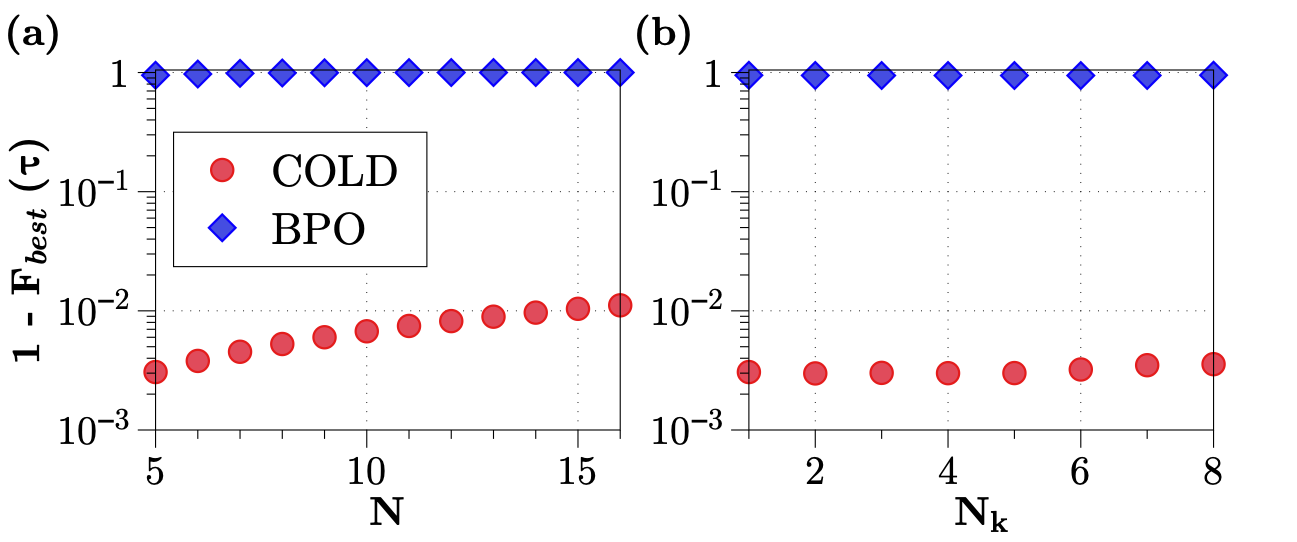
\includegraphics[width=\linewidth]{images/ScalingN.png} \caption[Plots of how final state fidelities scale using COLD and BPO for different system sizes and optimisable parameters.]{Scaling of fidelities in the annealing protocol for the Ising model with (a) system size $N$ and (b) optimisation parameters $N_k$ at driving time $\tau=10^{-2}J_0^{-1}$. Plots show a comparison between \acrref{BPO} (blue diamonds) and \acrref{COLD} (red circles).  In (a) we see that the \acrref{COLD} fidelity decreases as a function of $N$ but remains quite high when compared to \acrref{BPO} while (b) shows the non-existent improvement for both \acrref{BPO} and \acrref{COLD} with an increasing number of parameters in the $N=5$ spin case. Plotted best fidelities are obtained across 500 optimisations. Figure reproduced from \cite{cepaite_cold_2023}.}\label{fig:ising_scalingN}
\end{figure}

\begin{figure}[h]
    \centering
    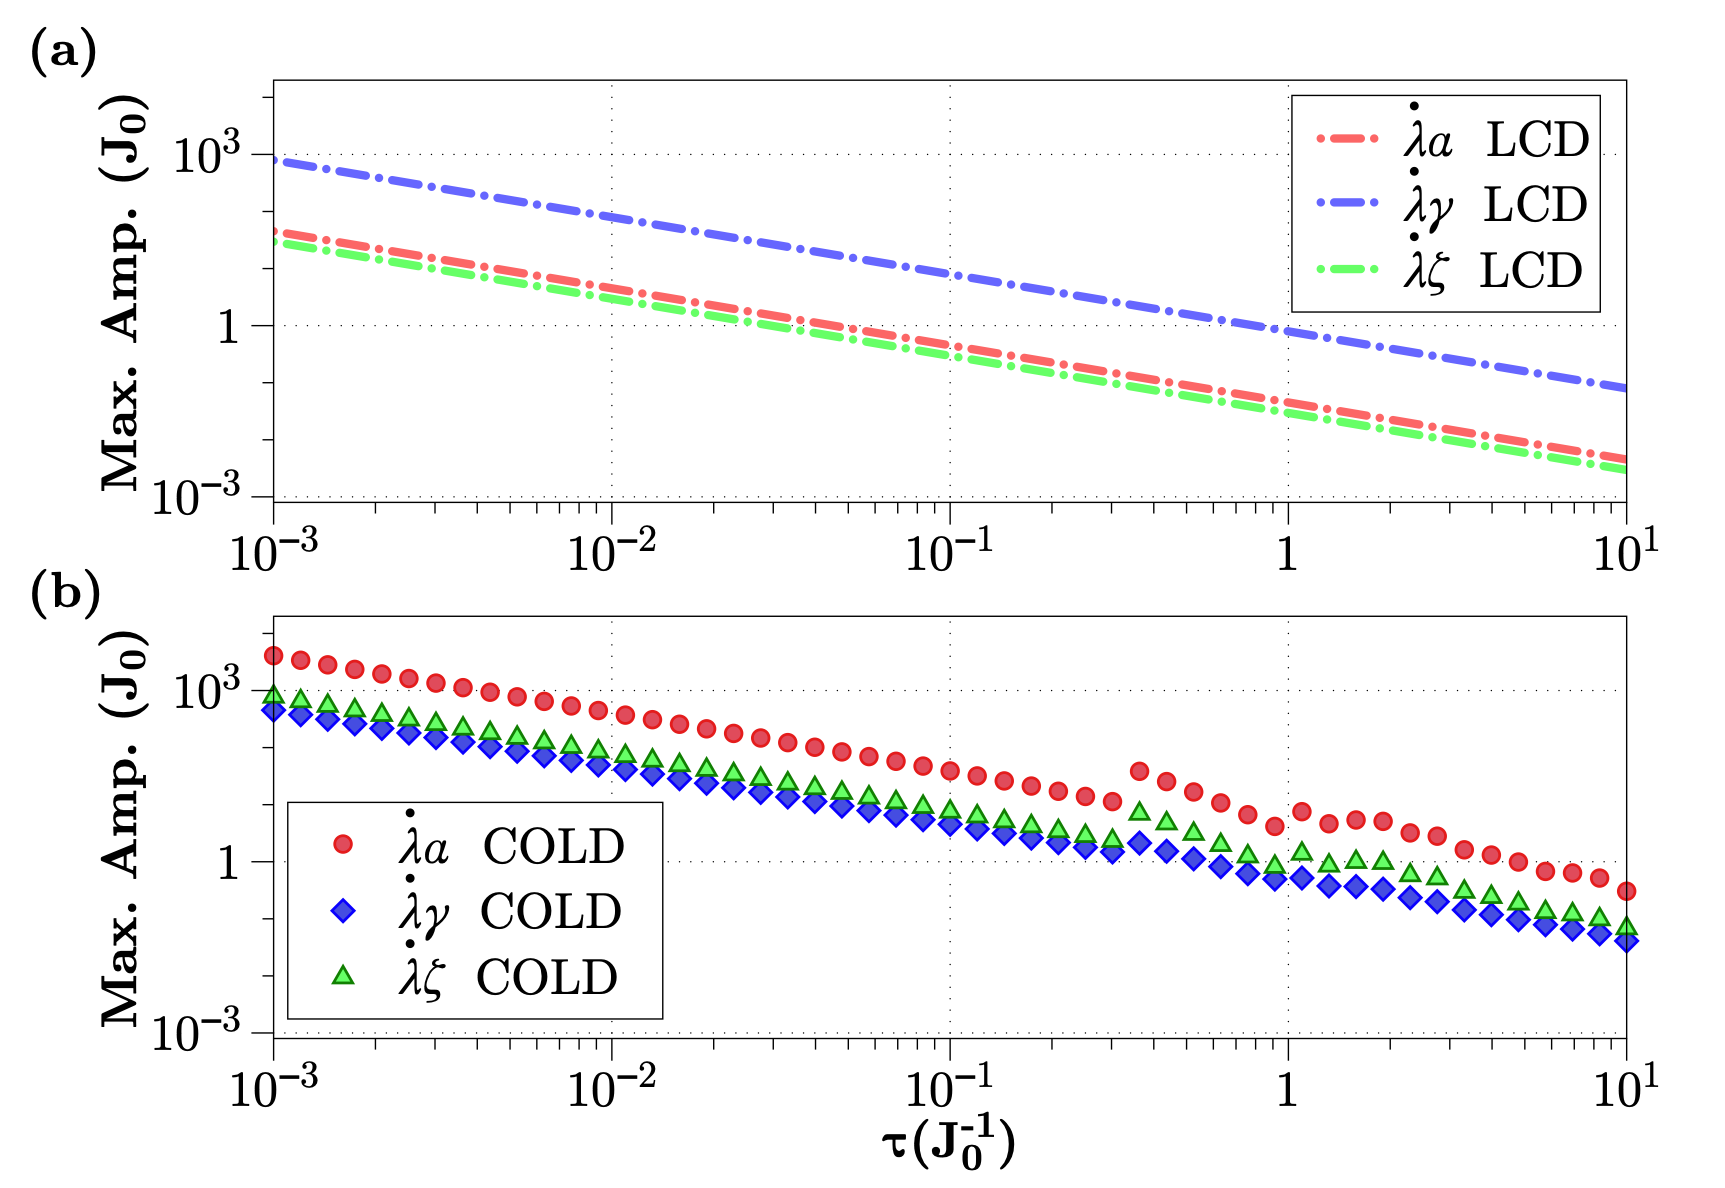
\includegraphics[width=0.8\linewidth]{images/MaxAmp.png} \caption[Plots of maximum amplitudes of LCD drives for the Ising spin chain.]{Figure reproduced from \cite{cepaite_cold_2023}.}\label{fig:ising_maxamp}
\end{figure}

\chapter{More details and plots for the higher order AGP chapter}\label{app:higher_order_AGP}

\begin{figure}[t]
    \centering
    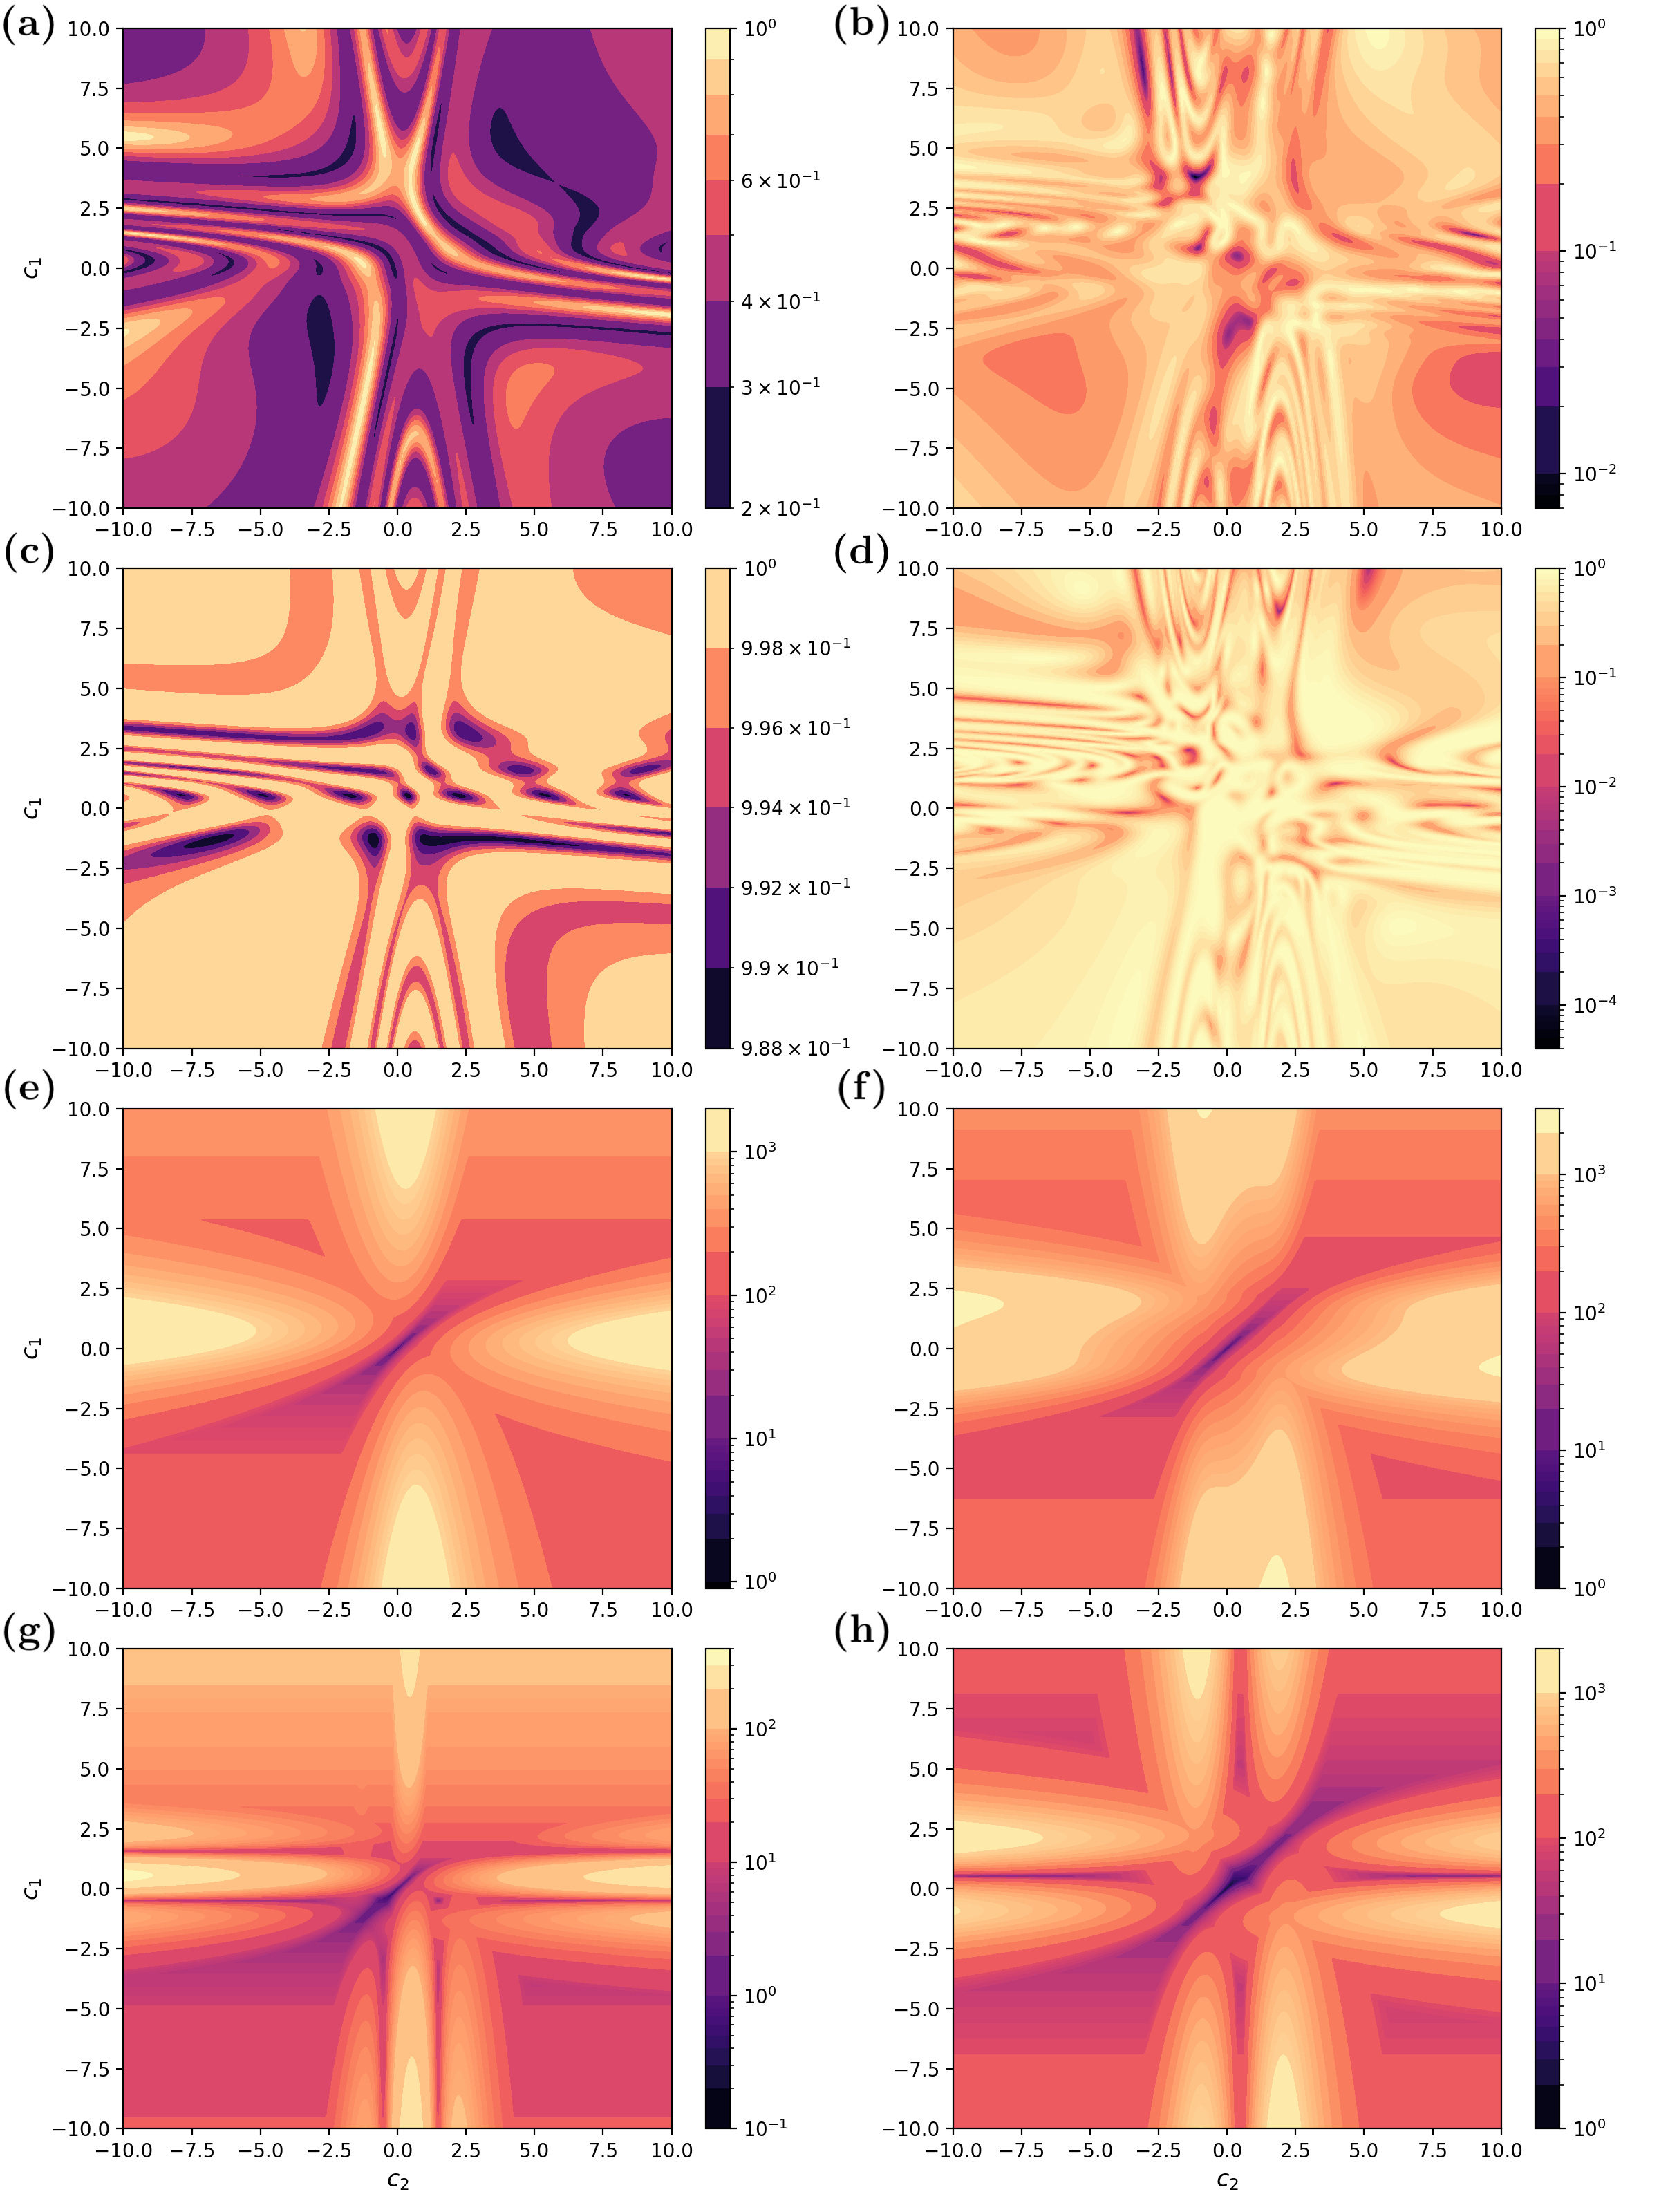
\includegraphics[width=0.8\linewidth]{images/ghz_contour_maximums.png} \caption[Contour plots of cost function landscapes for GHZ state preparation in frustrated spin systems (maximum amplitude cost function).]{Contour plots at $\tau = 0.1 J_0^{-1}$ of different cost function values for GHZ state preparation for parameters $c_1, c_2 \in [-10,10]$ and a \acrref{GRAPE} control pulse. In (a) and (b) we plot $C_{\rm F}$ in the cases where \acrref{FO} and \acrref{SO} \acrref{COLD} is applied respectively. Then, in (c-d) we do the same for $C_{T_3}$, with \acrref{FO} \acrref{COLD} plotted in (c) and \acrref{SO} \acrref{COLD} plotted in (d). (e-h) are then plots of the integral cost function $C_{\rm I}$ values for the same range of parameters. In (e) we plot $C_{\rm I, \alpha^{(1)}}$ when only \acrref{FO} \acrref{LCD} is considered, while in (f) we plot $C_{\rm I, \alpha^{(2)}}$ as described in the text. Then in (g) we plot $C_{\rm I, \gamma}$ and in (h) we plot $C_{\rm I, \zeta}$, corresponding to the \acrref{SO} terms. Note that each plot has its own color bar, as the color encodings and the value scaling in each plot is quite different.}\label{fig:ghz_contours_max_appendix}
\end{figure}

\begin{figure}[t]
    \centering
    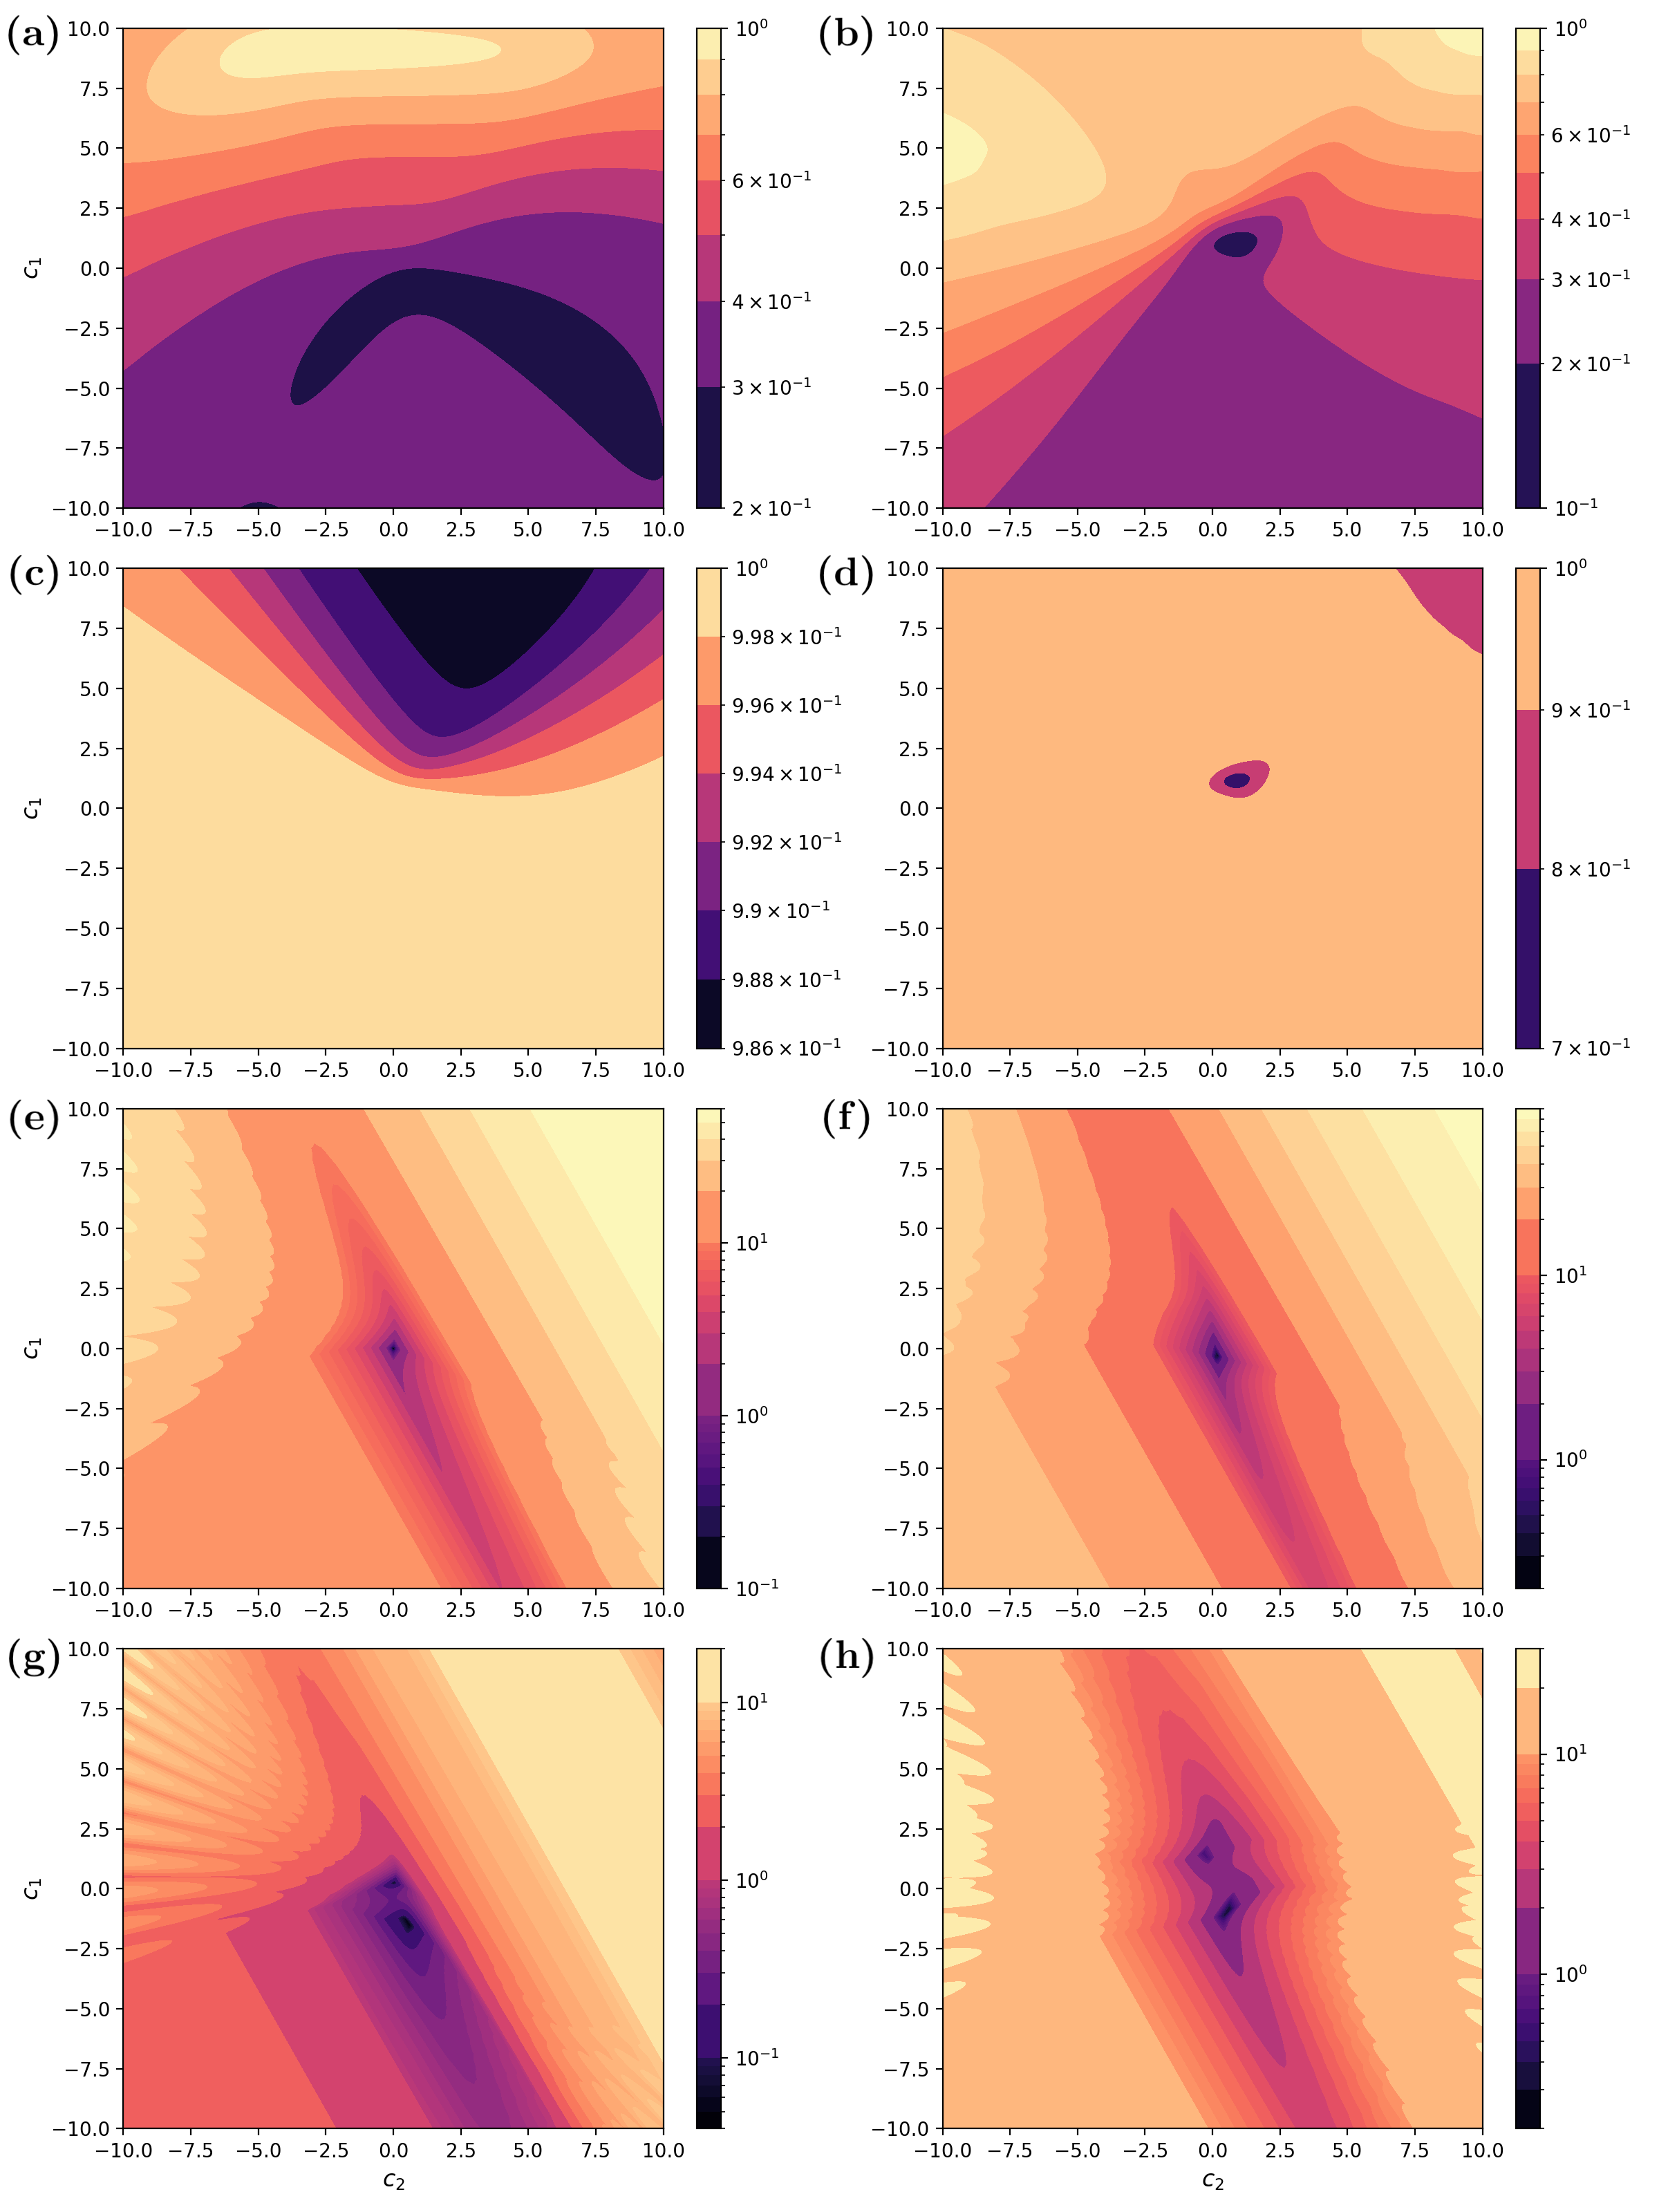
\includegraphics[width=0.8\linewidth]{images/final_plot_max_nogrape.png} \caption[Contour plots of cost function landscapes for GHZ state preparation in frustrated spin systems (maximum amplitude cost function) using a bare optimisation pulse.]{Contour plots at $\tau = 0.1 J_0^{-1}$ of different cost function values for GHZ state preparation for parameters $c_1, c_2 \in [-10,10]$ and a \acrref{GRAPE} control pulse. In (a) and (b) we plot $C_{\rm F}$ in the cases where \acrref{FO} and \acrref{SO} \acrref{COLD} is applied respectively. Then, in (c-d) we do the same for $C_{T_3}$, with \acrref{FO} \acrref{COLD} plotted in (c) and \acrref{SO} \acrref{COLD} plotted in (d). (e-h) are then plots of the integral cost function $C_{\rm I}$ values for the same range of parameters. In (e) we plot $C_{\rm I, \alpha^{(1)}}$ when only \acrref{FO} \acrref{LCD} is considered, while in (f) we plot $C_{\rm I, \alpha^{(2)}}$ as described in the text. Then in (g) we plot $C_{\rm I, \gamma}$ and in (h) we plot $C_{\rm I, \zeta}$, corresponding to the \acrref{SO} terms. Note that each plot has its own color bar, as the color encodings and the value scaling in each plot is quite different.}\label{fig:ghz_contours_max_noGRAPE}
\end{figure}

\begin{figure}[t]
    \centering
    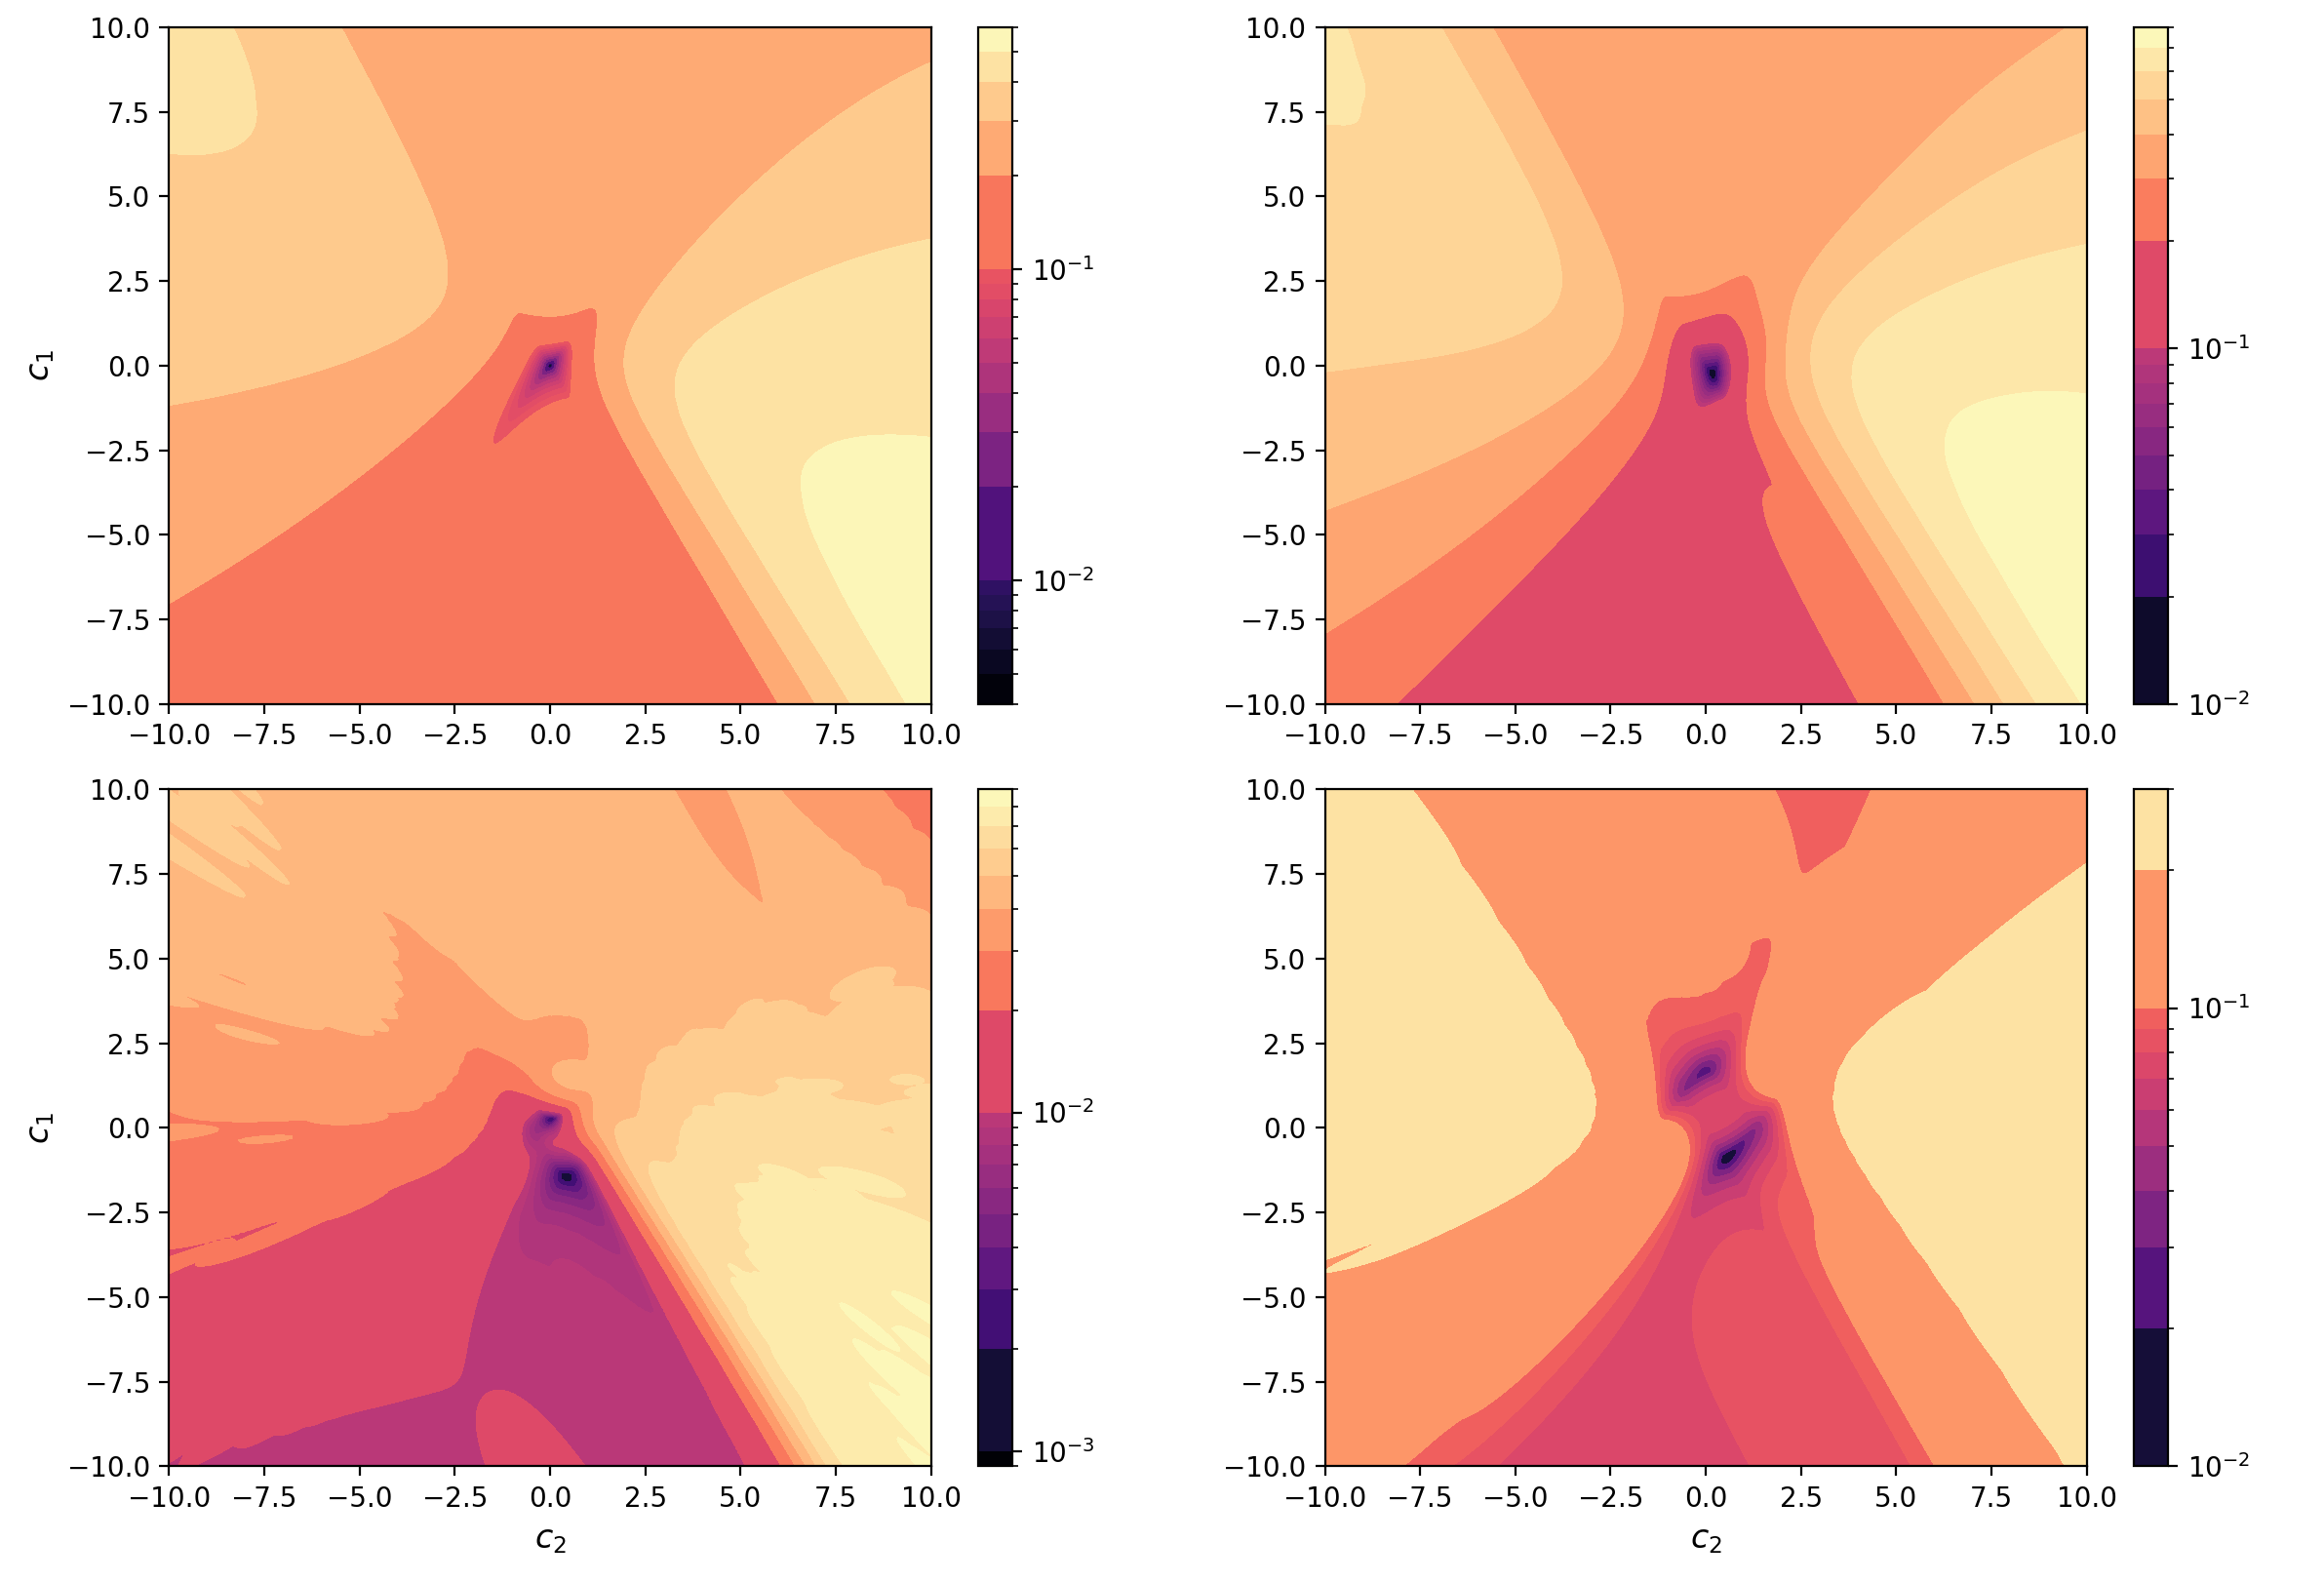
\includegraphics[width=0.8\linewidth]{images/final_plot_int_nogrape.png} \caption[Contour plots of cost function landscapes for GHZ state preparation in frustrated spin systems (maximum amplitude cost function) using a bare optimisation pulse.]{Contour plots at $\tau = 0.1 J_0^{-1}$ of different cost function values for GHZ state preparation for parameters $c_1, c_2 \in [-10,10]$ and a \acrref{GRAPE} control pulse. In (a) and (b) we plot $C_{\rm F}$ in the cases where \acrref{FO} and \acrref{SO} \acrref{COLD} is applied respectively. Then, in (c-d) we do the same for $C_{T_3}$, with \acrref{FO} \acrref{COLD} plotted in (c) and \acrref{SO} \acrref{COLD} plotted in (d). (e-h) are then plots of the integral cost function $C_{\rm I}$ values for the same range of parameters. In (e) we plot $C_{\rm I, \alpha^{(1)}}$ when only \acrref{FO} \acrref{LCD} is considered, while in (f) we plot $C_{\rm I, \alpha^{(2)}}$ as described in the text. Then in (g) we plot $C_{\rm I, \gamma}$ and in (h) we plot $C_{\rm I, \zeta}$, corresponding to the \acrref{SO} terms. Note that each plot has its own color bar, as the color encodings and the value scaling in each plot is quite different.}\label{fig:ghz_contours_int_noGRAPE}
\end{figure}
